\section*{Предисловие}

\subsection*{Почему два названия?}
\label{TwoTitles}

В 2014-2018 книга называлась ``Reverse Engineering для начинающих'', но я всегда подозревал что это слишком сужает аудиторию.

Люди от инфобезопасности знают о ``reverse engineering'', но я от них редко слышу слово ``ассемблер''.

Точно также, термин ``reverse engineering'' слишком незнакомый для общей аудитории программистов, но они знают про ``ассемблер''.

В июле 2018, для эксперимента, я заменил название на ``Assembly Language for Beginners''
и запостил ссылку на сайт Hacker News\footnote{\url{https://news.ycombinator.com/item?id=17549050}}, и книгу приняли, в общем, хорошо.

Так что, пусть так и будет, у книги будет два названия.

Хотя, я поменял второе название на ``Understanding Assembly Language'' (``Понимание языка ассемблера''), потому что кто-то уже написал книгу ``Assembly Language for Beginners''.
Также, люди говорят что ``для начинающих'' уже звучит немного саркастично для книги объемом в \textasciitilde{}1000 страниц.

Книги отличаются только названием, именем файла (UAL-XX.pdf и RE4B-XX.pdf), URL-ом и парой первых страниц.

\subsection*{О reverse engineering}

У термина \q{\gls{reverse engineering}} несколько популярных значений:
1) исследование скомпилированных
программ; 2) сканирование трехмерной модели для последующего копирования;
3) восстановление структуры СУБД. Настоящий сборник заметок
связан с первым значением.

\subsection*{Желательные знания перед началом чтения}

Очень желательно базовое знание \ac{PL} Си.
Рекомендуемые материалы: \myref{CCppBooks}.

\subsection*{Упражнения и задачи}

\dots 
все перемещены на отдельный сайт: \url{http://challenges.re}.

\subsection*{Об авторе}
\begin{tabularx}{\textwidth}{ l X }

\raisebox{-\totalheight}{
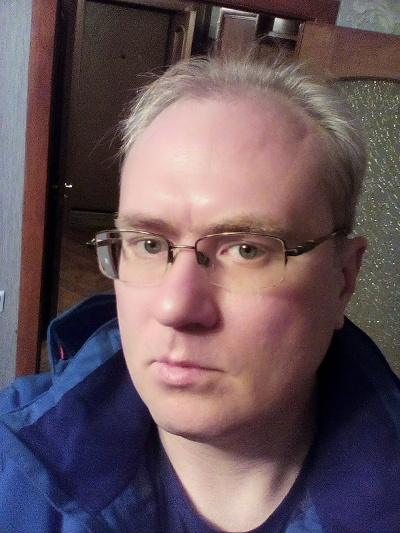
\includegraphics[scale=0.60]{Dennis_Yurichev.jpg}
}

&
Денис Юричев~--- опытный reverse engineer и программист.
С ним можно контактировать по емейлу: \textbf{\EMAIL{}}. % или по Skype: \textbf{dennis.yurichev}.

% FIXME: no link. \tablefootnote doesn't work
\end{tabularx}

% subsections:
\subsection*{%
	\RU{Отзывы об этой книге}%
	\EN{Praise for this book}%
	\ES{Elogios para}% TBT
	\PTBRph{}%
	\DE{Lob für}% TBT
	\PLph{}%
	\ITAph{}%
	\FR{Éloges de ce livre}%
	\JPN{賛辞}% TBT
}

\begin{itemize}

\item \q{Now that Dennis Yurichev has made this book free (libre), it is a contribution to the world of free knowledge and free education.} Richard M. Stallman,
\EN{GNU founder, software freedom activist.}
\RU{Основатель GNU, активист в области свободного ПО.}
\FR{Fondateur de GNU, militant pour la liberté des logiciels}
\JPN{GNU創設者、自由なソフトウェアの活動家}

% expanded URLs to make it more robust for printouts. In electronic editions people will click anyway, so tracking will keep working
\item \q{It's very well done .. and for free .. amazing.}\footnote{\href{http://go.yurichev.com/17095}{twitter.com/daniel\_bilar/status/436578617221742593}} Daniel Bilar, Siege Technologies, LLC.

\item \q{... excellent and free}\footnote{\href{http://go.yurichev.com/17096}{twitter.com/petefinnigan/status/400551705797869568}} Pete Finnigan,%
	\RU{гуру по безопасности}%
	\ES{gur\'u de seguridad en}%
	\PTBRph{}%
	\DE{Security-Guru}%
	\PLph{}%
	\ITAph{}
	\FR{gourou de la sécurité}
    \JPN{セキュリティグル}
\oracle
	\EN{security guru}.

\item \q{... [the] book is interesting, great job!} Michael Sikorski,
	\RU{автор книги}%
	\EN{author of}%
	\ES{autor de}%
	\PTBRph{}%
	\DE{Autor von}%
	\PLph{}%
	\ITAph{}
	\FR{auteur de}
	\JPN{以下の著作の著者です}
\IT{Practical Malware Analysis: The Hands-On Guide to Dissecting Malicious Software}.

\item \q{... my compliments for the very nice tutorial!} Herbert Bos,
	\RU{профессор университета}%
	\EN{full professor at the}%
	\ES{catedr\'atico de tiempo completo en la}%
	\PTBRph{}%
	\DE{Professor an der}%
	\PLph{}%
	\ITAph{}
	\FR{professeur à temps complet à}
	\JPN{教授}
Vrije Universiteit Amsterdam,
	\RU{соавтор}%
	\EN{co-author of}%
	\ES{coautor de}%
	\PTBRph{}%
	\DE{Co-Autor von}%
	\PLph{}%
	\ITAph{}
	\FR{co-auteur de}
	\JPN{共著者}
\IT{Modern Operating Systems (4th Edition)}.

\item \q{... It is amazing and unbelievable.} Luis Rocha, CISSP / ISSAP, Technical Manager, Network \& Information Security at Verizon Business.

\item \q{Thanks for the great work and your book.} Joris van de Vis,
	\RU{специалист по}%
	\ES{especialista en}%
	\PTBRph{}%
	\DE{Spezialist bei}%
	\PLph{}%
	\ITAph{}
	\FR{spécialiste}
SAP Netweaver \& Security
	\EN{specialist}.
	\JPN{スペシャリスト}

\item \q{... [a] reasonable intro to some of the techniques.}\footnote{\href{http://go.yurichev.com/17099}{reddit}} Mike Stay,
	\RU{преподаватель в}%
	\EN{teacher at the}%
	\ES{profesor en el}%
	\PTBRph{}%
	\DE{Professor an der}%
	\PLph{}%
	\ITAph{}
	\FR{professeur au}
	\JPN{教授}
Federal Law Enforcement Training Center, Georgia, US.

\item \q{I love this book! I have several students reading it at the moment, [and] plan to use it in graduate course.}\footnote{\href{http://go.yurichev.com/17097}{twitter.com/sergeybratus/status/505590326560833536}}
	\RU{Сергей Братусь}%
	\EN{Sergey Bratus}%
	\ES{Sergey Bratus}%
	\PTBRph{}%
	\DE{Sergey Bratus}%
	\PLph{}%
	\ITAph{}
	\FR{Sergey Bratus},
	\JPN{セルゲイブラウス}
Research Assistant Professor
	\RU{в отделе Computer Science в}%
	\EN{at the Computer Science Department at}%
	\ES{en el Departamento de Ciencias de la Computaci\'on en}%
	\PTBRph{}%
	\DE{an der Fakultät für Computer Science}
	\PLph{}%
	\ITAph{}
	\FR{dans le Département Informatique du}
Dartmouth College
	\JPN{コンピュータサイエンス学部}

\item \q{Dennis @Yurichev has published an impressive (and free!) book on reverse engineering}\footnote{\href{http://go.yurichev.com/17098}{twitter.com/TanelPoder/status/524668104065159169}} Tanel Poder,
	\RU{эксперт по настройке производительности Oracle RDBMS}%
	\EN{Oracle RDBMS performance tuning expert}%
	\ES{experto en afinaci\'on de rendimiento de Oracle RDBMS}%
	\PTBRph{}%
	\DE{Oracle RDBMS Performacence-Tuning Experte}%
	\PLph{}
	\ITAph{}
	\FR{expert en optimisation des performances Oracle RDBMS}
	\JPN{オラクルRDBMSパフォーマンスチューニングエキスパート}.

\item \q{This book is a kind of Wikipedia to beginners...} Archer, Chinese Translator, IT Security Researcher.

\RU{\item \q{Прочел Вашу книгу~--- отличная работа, рекомендую на своих курсах студентам
в качестве учебного пособия}. Николай Ильин, преподаватель в ФТИ НТУУ \q{КПИ} и DefCon-UA}

\item \q{[A] first-class reference for people wanting to learn reverse engineering. And it's free for all.} Mikko Hyppönen, F-Secure.

\end{itemize}

\ifdefined\RUSSIAN
\newcommand{\PeopleMistakesInaccuraciesRusEng}{Станислав \q{Beaver} Бобрицкий, Александр Лысенко, Александр \q{Solar Designer} Песляк, Федерико Рамондино, Марк Уилсон, Ксения Галинская, Разихова Мейрамгуль Кайратовна, Анатолий Прокофьев, Костя Бегунец, Валентин ``netch'' Нечаев, Александр Плахов, Артем Метла, Александр Ястребов, Влад Головкин\footnote{goto-vlad@github}}
\else
\newcommand{\PeopleMistakesInaccuraciesRusEng}{Stanislav \q{Beaver} Bobrytskyy, Alexander Lysenko, Alexander \q{Solar Designer} Peslyak, Federico Ramondino, Mark Wilson, Xenia Galinskaya, Razikhova Meiramgul Kayratovna, Anatoly Prokofiev, Kostya Begunets, Valentin ``netch'' Nechayev, Aleksandr Plakhov, Artem Metla, Alexander Yastrebov, Vlad Golovkin\footnote{goto-vlad@github}}
\fi

\newcommand{\PeopleMistakesInaccuracies}{\PeopleMistakesInaccuraciesRusEng{}, Shell Rocket, Zhu Ruijin, Changmin Heo, Vitor Vidal, Stijn Crevits, Jean-Gregoire Foulon\footnote{\url{https://github.com/pixjuan}}, Ben L., Etienne Khan, Norbert Szetei\footnote{\url{https://github.com/73696e65}}, Marc Remy, Michael Hansen, Derk Barten, The Renaissance\footnote{\url{https://github.com/TheRenaissance}}, Hugo Chan.}

\newcommand{\PeopleItalianTranslators}{Federico Ramondino\footnote{\url{https://github.com/pinkrab}},
Paolo Stivanin\footnote{\url{https://github.com/paolostivanin}}, twyK}

\newcommand{\PeopleFrenchTranslators}{Florent Besnard\footnote{\url{https://github.com/besnardf}}, Marc Remy\footnote{\url{https://github.com/mremy}}, Baudouin Landais, Téo Dacquet\footnote{\url{https://github.com/T30rix}}, BlueSkeye@GitHub\footnote{\url{https://github.com/BlueSkeye}}}

\newcommand{\PeopleGermanTranslators}{Dennis Siekmeier\footnote{\url{https://github.com/DSiekmeier}},
Julius Angres\footnote{\url{https://github.com/JAngres}}, Dirk Loser\footnote{\url{https://github.com/PolymathMonkey}}, Clemens Tamme}

\newcommand{\PeopleSpanishTranslators}{Diego Boy, Luis Alberto Espinosa Calvo, Fernando Guida, Diogo Mussi, Patricio Galdames}

\newcommand{\PeoplePTBRTranslators}{Thales Stevan de A. Gois, Diogo Mussi}

\newcommand{\PeoplePolishTranslators}{Kateryna Rozanova, Aleksander Mistewicz, Wiktoria Lewicka}

\newcommand{\PeopleJapaneseTranslators}{shmz@github\footnote{\url{https://github.com/shmz}}}

\newcommand{\FNGithubContributors}{\footnote{\url{https://github.com/DennisYurichev/RE-for-beginners/graphs/contributors}}}

\EN{\subsection*{Thanks}

For patiently answering all my questions: Slava \q{Avid} Kazakov, SkullC0DEr.

For sending me notes about mistakes and inaccuracies: \PeopleMistakesInaccuracies{}

For helping me in other ways:
Andrew Zubinski,
Arnaud Patard (rtp on \#debian-arm IRC),
noshadow on \#gcc IRC,
Aliaksandr Autayeu,
Mohsen Mostafa Jokar.

For translating the book into Simplified Chinese:
Antiy Labs (\href{http://antiy.cn}{antiy.cn}), Archer.

For translating the book into Korean: Byungho Min.

For translating the book into Dutch: Cedric Sambre (AKA Midas).

For translating the book into Spanish: \PeopleSpanishTranslators{}.

For translating the book into Portuguese: \PeoplePTBRTranslators{}.

For translating the book into Italian: \PeopleItalianTranslators{}.

For translating the book into French: \PeopleFrenchTranslators{}.

For translating the book into German: \PeopleGermanTranslators{}.

For translating the book into Polish: \PeoplePolishTranslators{}.

For translating the book into Japanese: \PeopleJapaneseTranslators{}.

For proofreading:
Alexander \q{Lstar} Chernenkiy,
Vladimir Botov,
Andrei Brazhuk,
Mark ``Logxen'' Cooper, Yuan Jochen Kang, Mal Malakov, Lewis Porter, Jarle Thorsen, Hong Xie.

Vasil Kolev\footnote{\url{https://vasil.ludost.net/}} did a great amount of work in proofreading and correcting many mistakes.

For illustrations and cover art: Andy Nechaevsky.

Thanks also to all the folks on github.com who have contributed notes and corrections\FNGithubContributors{}.

Many \LaTeX\ packages were used: I would like to thank the authors as well.

\subsubsection*{Donors}

Those who supported me during the time when I wrote significant part of the book:

\input{donors}

Thanks a lot to every donor!
}
\ES{\subsection*{Agradecimientos}

Por contestar pacientemente a todas mis preguntas: Slava \q{Avid} Kazakov, SkullC0DEr.

Por enviarme notas acerca de errores e inexactitudes: \PeopleMistakesInaccuracies{}.

Por ayudarme de otras formas:
Andrew Zubinski,
Arnaud Patard (rtp en \#debian-arm IRC),
noshadow en \#gcc IRC,
Aliaksandr Autayeu,
Mohsen Mostafa Jokar.

Por traducir el libro a Chino Simplificado:
Antiy Labs (\href{http://antiy.cn}{antiy.cn}), Archer.

Por traducir el libro a Coreano: Byungho Min.

\ESph{}: Cedric Sambre (AKA Midas).

\ESph{}: \PeopleSpanishTranslators{}.

\ESph{}: \PeoplePTBRTranslators{}.

\ESph{}: \PeopleItalianTranslators{}.

\ESph{}: \PeopleFrenchTranslators{}.

\DEph{}: \PeopleGermanTranslators{}.

\ac{TBT}: \PeoplePolishTranslators{}.

% TBT
%For translating the book into Japanese: \PeopleJapaneseTranslators{}.

\ES{Por correcci\'on de pruebas}%
Alexander \q{Lstar} Chernenkiy,
Vladimir Botov,
Andrei Brazhuk,
Mark ``Logxen'' Cooper, Yuan Jochen Kang, Mal Malakov, Lewis Porter, Jarle Thorsen, Hong Xie.

Vasil Kolev\footnote{\url{https://vasil.ludost.net/}} realiz\'o una gran cantidad de trabajo en correcci\'on de pruebas y correcci\'on de muchos errores.

Por las ilustraciones y el arte de la portada: Andy Nechaevsky.

Gracias a toda la gente en github.com que ha contribuido con notas y correcciones\FNGithubContributors{}.

Muchos paquetes de \LaTeX\ fueron utiliados: quiero agradecer tambi\'en a sus autores.

\subsubsection*{Donadores}

Aquellos que me apoyaron durante el tiempo que escrib\'i una parte significativa del libro:

\input{donors}

!`Gracias a cada donante!

}
\NL{\subsection*{Dankwoord}

Voor al mijn vragen geduldig te beantwoorden: Slava \q{Avid} Kazakov, SkullC0DEr.

Om me nota\'s over fouten en onnauwkeurigheden toe te sturen: \PeopleMistakesInaccuracies{}.

Om me te helpen op andere manieren:
Andrew Zubinski,
Arnaud Patard (rtp op \#debian-arm IRC),
noshadow op \#gcc IRC,
Aliaksandr Autayeu, Mohsen Mostafa Jokar.

Om het boek te vertalen naar het Vereenvoudigd Chinees:
Antiy Labs (\href{http://antiy.cn}{antiy.cn}), Archer.

Om dit boek te vertalen in het Koreaans: Byungho Min.

\NLph{}: Cedric Sambre (AKA Midas).

\NLph{}: \PeopleSpanishTranslators{}.

\NLph{}: \PeoplePTBRTranslators{}.

\NLph{}: \PeopleItalianTranslators{}.

\NLph{}: \PeopleFrenchTranslators{}.

\NLph{}: \PeopleGermanTranslators{}.

\ac{TBT}: \PeoplePolishTranslators{}.

% TBT
%For translating the book into Japanese: \PeopleJapaneseTranslators{}.

Voor proofreading:
Alexander \q{Lstar} Chernenkiy,
Vladimir Botov,
Andrei Brazhuk,
Mark ``Logxen'' Cooper, Yuan Jochen Kang, Mal Malakov, Lewis Porter, Jarle Thorsen, Hong Xie.

Vasil Kolev\footnote{\url{https://vasil.ludost.net/}}, voor het vele werk in proofreading en het verbeteren van vele fouten.

Voor de illustraties en cover art: Andy Nechaevsky.

Dank aan al de mensen op github.com die hebben nota\'s en correcties hebben bijgedragen\FNGithubContributors{}.

Veel \LaTeX\ packages zijn gebruikt. Ik zou de auteurs hiervan ook graag bedanken.

\subsubsection*{Donaties}

Zij die me gesteund hebben tijdens het schrijven van een groot deel van dit boek:

\input{donors}

Veel dank aan elke donor!
}
\RU{\subsection*{Благодарности}

Тем, кто много помогал мне отвечая на массу вопросов: Слава \q{Avid} Казаков, SkullC0DEr.

Тем, кто присылал замечания об ошибках и неточностях: \PeopleMistakesInaccuracies{}.

Просто помогали разными способами:
Андрей Зубинский,
Arnaud Patard (rtp на \#debian-arm IRC),
noshadow на \#gcc IRC,
Александр Автаев,
Mohsen Mostafa Jokar.

Переводчикам на китайский язык:
Antiy Labs (\href{http://antiy.cn}{antiy.cn}), Archer.

Переводчику на корейский язык: Byungho Min.

Переводчику на голландский язык: Cedric Sambre (AKA Midas).

Переводчикам на испанский язык: \PeopleSpanishTranslators{}.

Переводчикам на португальский язык: \PeoplePTBRTranslators{}.

Переводчикам на итальянский язык: \PeopleItalianTranslators{}.

Переводчикам на французский язык: \PeopleFrenchTranslators{}.

Переводчикам на немецкий язык: \PeopleGermanTranslators{}.

Переводчикам на польский язык: \PeoplePolishTranslators{}.

Переводчикам на японский язык: \PeopleJapaneseTranslators{}.

Корректорам:
Александр \q{Lstar} Черненький,
Владимир Ботов,
Андрей Бражук,
Марк ``Logxen'' Купер, Yuan Jochen Kang, Mal Malakov, Lewis Porter, Jarle Thorsen, Hong Xie.

Васил Колев\footnote{\url{https://vasil.ludost.net/}} сделал очень много исправлений и указал на многие ошибки.

За иллюстрации и обложку: Андрей Нечаевский.

И ещё всем тем на github.com кто присылал замечания и исправления\FNGithubContributors{}.

Было использовано множество пакетов \LaTeX. Их авторов я также хотел бы поблагодарить.

\subsubsection*{Жертвователи}

Тем, кто поддерживал меня во время написания этой книги:

\input{donors}

Огромное спасибо каждому!

}
\ITA{\subsection*{Ringraziamenti}

Per aver pazientemente risposto a tutte le mie domande: Slava \q{Avid} Kazakov, SkullC0DEr.

Per avermi inviato note riguardo i miei errori e le inaccuratezze: \PeopleMistakesInaccuracies{}.

Per avermi aiutato in altri modi:
Andrew Zubinski,
Arnaud Patard (rtp on \#debian-arm IRC),
noshadow on \#gcc IRC,
Aliaksandr Autayeu,
Mohsen Mostafa Jokar.

Per aver tradotto il libro in Cinese Semplificato:
Antiy Labs (\href{http://antiy.cn}{antiy.cn}), Archer.

Per la traduzione Coreana: Byungho Min.

Per la traduzione in Olandese: Cedric Sambre (AKA Midas).

Per la traduzione in Spagnolo: \PeopleSpanishTranslators{}.

Per la traduzione in Portoghese: \PeoplePTBRTranslators{}.

Per la traduzione Italiana: \PeopleItalianTranslators{}.

\ITAph{}: \PeopleFrenchTranslators{}.

\ITAph{}: \PeopleGermanTranslators{}.

\ac{TBT}: \PeoplePolishTranslators{}.

% TBT
%For translating the book into Japanese: \PeopleJapaneseTranslators{}.

Per la revisione:
Alexander \q{Lstar} Chernenkiy,
Vladimir Botov,
Andrei Brazhuk,
Mark ``Logxen'' Cooper, Yuan Jochen Kang, Mal Malakov, Lewis Porter, Jarle Thorsen, Hong Xie.

Vasil Kolev\footnote{\url{https://vasil.ludost.net/}} ha speso una notevole quantità di tempo per la revisione e la correzione di molti errori.

Per le illustrazioni e la copertina: Andy Nechaevsky.

Grazie inoltre a tutti quelli su github.com che hanno contribuito a note e correzioni\FNGithubContributors{}.

Sono stati usati molti pacchetti \LaTeX\ : vorrei ringraziare tutti gli autori di tali moduli.

\subsubsection*{Donatori}

Tutti quelli che mi hanno supportato durante il tempo in cui ho scritto la parte più significativa del libro:

\input{donors}

Grazie di cuore a tutti i donatori!
}
\FR{\subsection*{Remerciements}

Pour avoir patiemment répondu à toutes mes questions : Slava \q{Avid} Kazakov, SkullC0DEr.

Pour m'avoir fait des remarques par rapport à mes erreurs ou manques de précision : \PeopleMistakesInaccuracies{}.

Pour m'avoir aidé de toute autre manière :
Andrew Zubinski,
Arnaud Patard (rtp on \#debian-arm IRC),
noshadow on \#gcc IRC,
Aliaksandr Autayeu,
Mohsen Mostafa Jokar.

Pour avoir traduit le livre en chinois simplifié :
Antiy Labs (\href{http://antiy.cn}{antiy.cn}), Archer.

Pour avoir traduit le livre en coréen : Byungho Min.

Pour avoir traduit le livre en néerlandais : Cedric Sambre (AKA Midas).

Pour avoir traduit le livre en espagnol : \PeopleSpanishTranslators{}.

Pour avoir traduit le livre en portugais : \PeoplePTBRTranslators{}.

Pour avoir traduit le livre en italien : \PeopleItalianTranslators{}.

Pour avoir traduit le livre en français : \PeopleFrenchTranslators{}.

Pour avoir traduit le livre en allemand : \PeopleGermanTranslators{}.

Pour avoir traduit le livre en polonais: \PeoplePolishTranslators{}.

Pour avoir traduit le livre en japonais: \PeopleJapaneseTranslators{}.

Pour la relecture :
Alexander \q{Lstar} Chernenkiy,
Vladimir Botov,
Andrei Brazhuk,
Mark ``Logxen'' Cooper, Yuan Jochen Kang, Mal Malakov, Lewis Porter, Jarle Thorsen, Hong Xie.

Vasil Kolev\footnote{\url{https://vasil.ludost.net/}} a réalisé un gros travail de relecture et a corrigé beaucoup d'erreurs.

Pour les illustrations et la couverture : Andy Nechaevsky.

Merci également à toutes les personnes sur github.com qui ont contribué aux remarques et aux corrections\FNGithubContributors{}.

De nombreux packages \LaTeX\ ont été utilisé : j'aimerais également remercier leurs auteurs.

\subsubsection*{Donateurs}

Ceux qui m'ont sontenu lorsque j'écrivais le livre :

\input{donors}

Un énorme merci à chaque donateur !
}
\DE{\subsection*{Danksagung}

Für das geduldige Beantworten aller meiner Fragen: Slava \q{Avid} Kazakov, SkullC0DEr.

Für Anmerkungen über Fehler und Unstimmigkeiten: \PeopleMistakesInaccuracies{}.

Für die Hilfe in anderen Dingen:
Andrew Zubinski,
Arnaud Patard (rtp on \#debian-arm IRC),
noshadow on \#gcc IRC,
Aliaksandr Autayeu,
Mohsen Mostafa Jokar.

Für die Übersetzung des Buchs ins Vereinfachte Chinesisch:
Antiy Labs (\href{http://antiy.cn}{antiy.cn}), Archer.

Für die Übersetzung des Buchs ins Koreanische: Byungho Min.

Für die Übersetzung des Buchs ins Niederländische: Cedric Sambre (AKA Midas).

Für die Übersetzung des Buchs ins Spanische: \PeopleSpanishTranslators{}.

Für die Übersetzung des Buchs ins Portugiesische: \PeoplePTBRTranslators{}.

Für die Übersetzung des Buchs ins Italienische: \PeopleItalianTranslators{}.

Für die Übersetzung des Buchs ins Französische: \PeopleFrenchTranslators{}.

Für die Übersetzung des Buchs ins Deutsche: \PeopleGermanTranslators{}.

Für die Übersetzung des Buchs ins Polnische: \PeoplePolishTranslators{}.

Für die Übersetzung des Buchs ins Japanische: \PeopleJapaneseTranslators{}.

Für das Korrekturlesen:
Alexander \q{Lstar} Chernenkiy,
Vladimir Botov,
Andrei Brazhuk,
Mark ``Logxen'' Cooper, Yuan Jochen Kang, Mal Malakov, Lewis Porter, Jarle Thorsen, Hong Xie.

Vasil Kolev\footnote{\url{https://vasil.ludost.net/}} der unglaublich viel Arbeit in die Korrektur vieler Fehler investiert hat.

Für Abbildungen und die Cover-Gestaltung: Andy Nechaevsky.

Danke auch an alle, die auf github.com Anmerkungen und Korrekturen eingebracht haben\FNGithubContributors{}.

Es wurden viele \LaTeX\-Pakete genutzt: Vielen Dank an deren Autoren.

\subsubsection*{Donors}

Dank an diejenigen die mich während der Zeit in der ich wichtige Teile des Buchs geschrieben habe
unterstützt haben:

\input{donors}

Vielen Dank an alle Spender!
}
%\CN{% !TEX program = XeLaTeX
% !TEX encoding = UTF-8
\documentclass[UTF8,nofonts]{ctexart}
\setCJKmainfont[BoldFont=STHeiti,ItalicFont=STKaiti]{STSong}
\setCJKsansfont[BoldFont=STHeiti]{STXihei}
\setCJKmonofont{STFangsong}

\begin{document}

%daveti: translated on Dec 28, 2016
%NOTE: above is needed for MacTex.

\subsection*{感谢 Thanks}

耐心回答我每一个问题的人: Slava \q{Avid} Kazakov, SkullC0DEr.

为本书勘误的人: \PeopleMistakesInaccuracies{}.

其他形式帮忙的人:
Andrew Zubinski,
Arnaud Patard (rtp on \#debian-arm IRC),
noshadow on \#gcc IRC,
Aliaksandr Autayeu,
Mohsen Mostafa Jokar.

中文翻译~\footnote{译者语:可能是之前的那个epub版本,反正不是俺}:
Antiy Labs (\href{http://antiy.cn}{antiy.cn}), Archer.

韩语翻译: Byungho Min.

荷兰语翻译: Cedric Sambre (AKA Midas).

西班牙语翻译: \PeopleSpanishTranslators{}.

葡萄牙语翻译: \PeoplePTBRTranslators{}.

意大利语翻译: \PeopleItalianTranslators{}.

法语翻译: \PeopleFrenchTranslators{}.

德语翻译: \PeopleGermanTranslators{}.

\ac{TBT}: \PeoplePolishTranslators{}.

% TBT
%For translating the book into Japanese: \PeopleJapaneseTranslators{}.

试读的人:
Alexander \q{Lstar} Chernenkiy,
Vladimir Botov,
Andrei Brazhuk,
Mark ``Logxen'' Cooper, Yuan Jochen Kang, Mal Malakov, Lewis Porter, Jarle Thorsen, Hong Xie.

Vasil Kolev\footnote{\url{https://vasil.ludost.net/}}做了大量的试读和纠错工作。

封面插曲艺术设计: Andy Nechaevsky.

感谢github.com所有提出建议或者纠错的人\FNGithubContributors{}.

本书使用了很多\LaTeX\ 包: 我也感谢这些软件的作者.

\subsubsection*{捐献者 Donors}

那些在我写书时提供各种帮助的人:

\input{donors}

感谢你们的每一份捐助!

\end{document}
}
\JPN{\subsection*{謝辞}

忍耐強く質問に答えてくれた方々:Slava \q{Avid} Kazakov, SkullC0DEr

ミスや不正確な記述を指摘してくれた方々:\PeopleMistakesInaccuracies{}

他に手助けしてくれた方々:
Andrew Zubinski,
Arnaud Patard (rtp on \#debian-arm IRC),
noshadow on \#gcc IRC,
Aliaksandr Autayeu,
Mohsen Mostafa Jokar.

簡体字中国語への翻訳:Antiy Labs(\href{http://antiy.cn}{antiy.cn})、Archer

韓国語への翻訳:Byungho Min

オランダ語への翻訳:Cedric Sambre(AKA Midas)

スペイン語への翻訳: \PeopleSpanishTranslators{}

ポルトガル語への翻訳:\PeoplePTBRTranslators{}

イタリア語への翻訳:\PeopleItalianTranslators{}

フランス語への翻訳:\PeopleFrenchTranslators{}

ドイツ語への翻訳:\PeopleGermanTranslators{}

ポーランド語への翻訳:\PeoplePolishTranslators{}

日本語への翻訳:\PeopleJapaneseTranslators{}.

校正者:
Alexander \q{Lstar} Chernenkiy,
Vladimir Botov,
Andrei Brazhuk,
Mark ``Logxen'' Cooper, Yuan Jochen Kang, Mal Malakov, Lewis Porter, Jarle Thorsen, Hong Xie.

Vasil Kolev\footnote{\url{https://vasil.ludost.net/}} は大量の校正とミスを訂正してくれました。

イラストとカバーアート:Andy Nechaevsky

github.comでフォークして指摘や訂正してくれたすべての方々に感謝します:\FNGithubContributors{}

\LaTeX\ パッケージをたくさん使っています:パッケージの作者にも合わせて感謝します

\subsubsection*{ドナー}

本の大半を執筆中にサポートしてくれた方々:

\input{donors}

ドナーの方すべてに感謝します!
}

\subsection*{mini-ЧаВО}

\par Q: Что необходимо знать перед чтением книги?
\par A: Желательно иметь базовое понимание Си/Си++.

\par Q: Должен ли я изучать сразу x86/x64/ARM и MIPS? Это не многовато?
\par A: Думаю, для начала, вы можете читать только о x86/x64, пропуская/пролистывая части о ARM/MIPS.

\par Q: Возможно ли купить русскую/английскую бумажную книгу?
\par A: К сожалению нет, пока ни один издатель не заинтересовался в издании русской или английской версии.
А пока вы можете распечатать/переплести её в вашем любимом копи-шопе или копи-центре.

\par Q: Существует ли версия epub/mobi?
\par A: Книга очень сильно завязана на специфические для TeX/LaTeX хаки, поэтому преобразование в HTML (epub/mobi это набор HTML)
легким не будет.

\par Q: Зачем в наше время нужно изучать язык ассемблера?
\par A: Если вы не разработчик \ac{OS}, вам наверное не нужно писать на ассемблере: современные компиляторы (2010-ые) оптимизируют код намного лучше человека
\footnote{Очень хороший текст на эту тему: \InSqBrackets{\AgnerFog}}.

К тому же, современные \ac{CPU} это крайне сложные устройства и знание ассемблера вряд ли
поможет узнать их внутренности.

Но все-таки остается по крайней мере две области, где знание ассемблера может хорошо помочь:
1) исследование malware (\IT{зловредов}) с целью анализа; 2) лучшее понимание
вашего скомпилированного кода в процессе отладки.
Таким образом, эта книга предназначена для тех, кто хочет скорее понимать ассемблер,
нежели писать на нем, и вот почему здесь масса примеров, связанных с результатами
работы компиляторов.

\par Q: Я кликнул на ссылку внутри PDF-документа, как теперь вернуться назад?
\par A: В Adobe Acrobat Reader нажмите сочетание Alt+LeftArrow. В Evince кликните на ``<''.

\par Q: Могу ли я распечатать эту книгу? Использовать её для обучения?
\par A: Конечно, поэтому книга и лицензирована под лицензией Creative Commons (CC BY-SA 4.0).

\par Q: Почему эта книга бесплатная? Вы проделали большую работу. Это подозрительно, как и многие другие бесплатные вещи.
\par A: По моему опыту, авторы технической литературы делают это, в основном ради саморекламы. Такой работой заработать приличные деньги невозможно.

\par Q: Как можно найти работу reverse engineer-а?
\par A: На reddit, посвященному RE\FNURLREDDIT, время от времени бывают hiring thread (\RedditHiringThread{}).
Посмотрите там.

В смежном субреддите \q{netsec} имеется похожий тред: \NetsecHiringThread{}.

% TODO \ref...
\myindex{LISP}
\par Q: Как научиться программированию вообще?
\par A: Если вы можете хорошо освоить и Си и LISP, это делает жизнь программиста значительно легче.
Я бы порекомендовал решать задачи из [\KRBook] и \ac{SICP}.

\par Q: У меня есть вопрос...
\par A: Напишите мне его емейлом (\EMAIL).


\subsection*{Как научиться программированию}

Многие люди спрашивают об этом.

Легких путей нет, но есть пути быстрые и эффективные.

Из моего опыта, это просто: решать задачи из:

\begin{itemize}
\item \KRBook
\item Харольд Абельсон, Джеральд Сассман -- Структура и интерпретация компьютерных программ
\item \TAOCP
\item Книги Никласа Вирта
\item \RobPikePractice
\end{itemize}

... на чистом Си и Лиспе.
В будущем, возможно, вы не будете использовать эти языки вообще.
Большинство коммерческих программистов не используют. Но опыт программирования на Си и Лиспе помогает очень сильно в 
долгосрочной перспективе.

Также, вы можете не читать сами книги, просто листайте, тогда, когда вы чувствуете, что вы не можете чего-то
понять для решения задачи.

В лучшем случае, это занимает годы, или всю жизнь, но это все же намного быстрее, чем метаться между очередными модными
штуками.

Успех этих книг вероятно связан с тем, что их авторы -- преподаватели, и весь материал был в начале отточен на студентах.

Насчет Лиспа, я бы рекомендовал Racket (диалект Scheme). Но это дело вкуса, так или иначе.

Некоторые люди говорят, что понимание ассемблера очень помогает, даже если вы не будете использовать его.
Это верно.
Но это уже путь для наиболее посвященных гиков, и для начала это можно отложить на будущее.

Также, очень частая проблема самоучек (включая автора этих строк), это то, что они слишком часто хватаются
за слишком трудные проблемы, пропуская более легкие.
Это большая ошибка.
Сравните со спортом или музыкой -- никто не начинает с попыток поднимать сразу 100 кг,
или же сразу пытаться играть Капризы Паганини.
Я бы сказал так -- браться за задачу можно тогда, когда вы зараннее, в уме, можете примерно прикинуть решение.

\begin{framed}
\begin{quotation}                                                                                                               I think the art of doing research consists largely of asking questions,
and sometimes answering them. Learn how to repeatedly pose miniquestions
that represent special cases of the big questions you are hoping to solve.

When you begin to explore some area, you take baby steps at first, building
intuition about that territory. Play with many small examples, trying to
get a complete understanding of particular parts of the general situation.

In that way you learn many properties that are true and many properties
that are false. That gives guidance about directions that are fruitful
versus directions to avoid.

Eventually your brain will have learned how to take larger and larger steps.
And shazam, you’ll be ready to take some giant steps and solve the big problem.

But don’t stop there! At this point you’ll be one of very few people in the
world who have ever understood your problem area so well. It will therefore
be your responsibility to discover what else is true, in the neighborhood
of that problem, using the same or similar methods to what your brain
can now envision. Take your results to their “natural boundary” (in a sense
analogous to the natural boundary where a function of a complex variable
ceases to be analytic).

My little book Surreal Numbers provides an authentic example of research
as it is happening. The characters in that story make false starts and
useful discoveries in exactly the same order as I myself made those false starts
and useful discoveries, when I first studied John Conway’s fascinating
axioms about number systems — his amazingly simple axioms that go
significantly beyond real-valued numbers.

(One of the characters in that book tends to succeed or fail by brute force
and patience; the other is more introspective, and able to see a bigger
picture. Both of them represent aspects of my own activities while doing
research. With that book I hoped to teach research skills “by osmosis”,
as readers observe a detailed case study.)

Surreal Numbers deals with a purely mathematical topic, not especially close
to computer science; it features algebra and logic, not algorithms.
When algorithms become part of the research, a beautiful new dimension
also comes into play: Algorithms can be implemented on computers!

I strongly recommend that you look for every opportunity to write programs
that carry out all or a part of whatever algorithms relate to your research.
In my experience the very act of writing such a program never fails to
deepen my understanding of the problem area.
\end{quotation}
\end{framed}

( Дональд Э. Кнут -- \url{https://theorydish.blog/2018/02/01/donald-knuth-on-doing-research/} )

Удачи!

\subsection*{О переводе на корейский язык}

В январе 2015, издательство Acorn в Южной Корее сделало много работы в переводе 
и издании моей книги (по состоянию на август 2014) на корейский язык.
Она теперь доступна на \href{http://go.yurichev.com/17343}{их сайте}.

\iffalse
\begin{figure}[H]
\centering
\includegraphics[scale=0.3]{acorn_cover.jpg}
\end{figure}
\fi

Переводил Byungho Min (\href{http://go.yurichev.com/17344}{twitter/tais9}).
Обложку нарисовал мой хороший знакомый художник Андрей Нечаевский
\href{http://go.yurichev.com/17023}{facebook/andydinka}.
Они также имеют права на издание книги на корейском языке.
Так что если вы хотите иметь \IT{настоящую} книгу на полке на корейском языке и
хотите поддержать мою работу, вы можете купить её.

\subsection*{О переводе на персидский язык (фарси)}

В 2016 году книга была переведена Mohsen Mostafa Jokar (который также известен иранскому сообществу по переводу руководства Radare\footnote{\url{http://rada.re/get/radare2book-persian.pdf}}).
Книга доступна на сайте издательства\footnote{\url{http://goo.gl/2Tzx0H}} (Pendare Pars).

Первые 40 страниц: \url{https://beginners.re/farsi.pdf}.

Регистрация книги в Национальной Библиотеке Ирана: \url{http://opac.nlai.ir/opac-prod/bibliographic/4473995}.

\subsection*{О переводе на китайский язык}

В апреле 2017, перевод на китайский был закончен китайским издательством PTPress. Они также имеют права на издание книги на китайском языке.

Она доступна для заказа здесь: \url{http://www.epubit.com.cn/book/details/4174}. Что-то вроде рецензии и история о переводе: \url{http://www.cptoday.cn/news/detail/3155}.

Основным переводчиком был Archer, перед которым я теперь в долгу.
Он был крайне дотошным (в хорошем смысле) и сообщил о большинстве известных ошибок и баг, что крайне важно для литературы вроде этой книги.
Я буду рекомендовать его услуги всем остальным авторам!

Ребята из \href{http://www.antiy.net/}{Antiy Labs} также помогли с переводом. \href{http://www.epubit.com.cn/book/onlinechapter/51413}{Здесь предисловие} написанное ими.

